\section{Pianificazione}
	
	Il gruppo EverBuilds ha deciso di pianificare il progetto in base alle scadenze prefissate in §1.5 dall'università e a quelle interne del gruppo.
	\\
	\\
	Di seguito le fasi di suddivisione del progetto:
	\begin{itemize}
		\item \textbf{\glock{individuazione degli strumenti} e \glock{analisi dei requisiti};}
		\item \textbf{\glock{analisi di dettaglio};}
		\item \textbf{\glock{progettazione architetturale};}
		\item \textbf{\glock{progettazione di dettaglio} e \glock{codifica};}
		\item \textbf{\glock{validazione} e \glock{collaudo}.}
	\end{itemize}
	Ognuna delle precedenti fasi verrà vista nel dettaglio suddividendole in attività e sotto-attività tramite descrizione delle stesse e collocamento nei rispettivi \glock{diagrammi di Gantt}, uno per fase.
	
\subsection{Individuazione degli strumenti e analisi dei requisiti}

	\textbf{periodo:} da 2020-12-05 a 2021-01-11 
	\begin{itemize}
		\item \textbf{\glock{Individuazione degli strumenti}:} vengono scelti da subito gli strumenti per la stesura dei documenti di cui Google Drive e Latex, inoltre viene scelto GitHub per la gestione della repository e Telegram assieme a Discord per la comunicazione;
		\item \textbf{Norme di Progetto:} con i medesimi strumenti viene steso il documento \glock{Norme di Progetto v1.00} indipendentemente dal \glock{capitolato} che sarà preso in appalto;
		\item \textbf{Studio di Fattibilità:} vengono analizzati tutti i capitolati proposti e scritto il documento “Studio di Fattibilità v1.00” tramite il quale verrà scelto il capitolato dal gruppo;
		\item \textbf{\glock{Analisi dei Requisiti}:} comincia una prima stesura del documento \glock{Analisi dei Requisiti} v1.00. Continuerà ad essere migliorato fino a poco prima della data di consegna. È incluso nell’attività un incontro con il proponente per consolidare i requisiti stesi fino a quel momento;
		\item \textbf{\glock{Piano di Progetto}:} redatto il \glock{Piano di Progetto} v1.00 per regolare le attività che il gruppo dovrà svolgere;
		\item \textbf{\glock{Piano di Qualifica}:} si redige \glock{Piano di Qualifica} v1.00;		
		\item \textbf{\glock{Glossario}:} si redige il \glock{Glossario} v1.00;
		\item \textbf{\glock{Lettera di Presentazione}:} si scrive un breve documento in cui il gruppo EverBuilds si propone per il \glock{capitolato} scelto.
	\end{itemize}  

	\subsubsection{Diagramma di Gantt: individuazione degli strumenti e analisi dei requisiti}
	
		\begin{figure}[H]
			\centering
			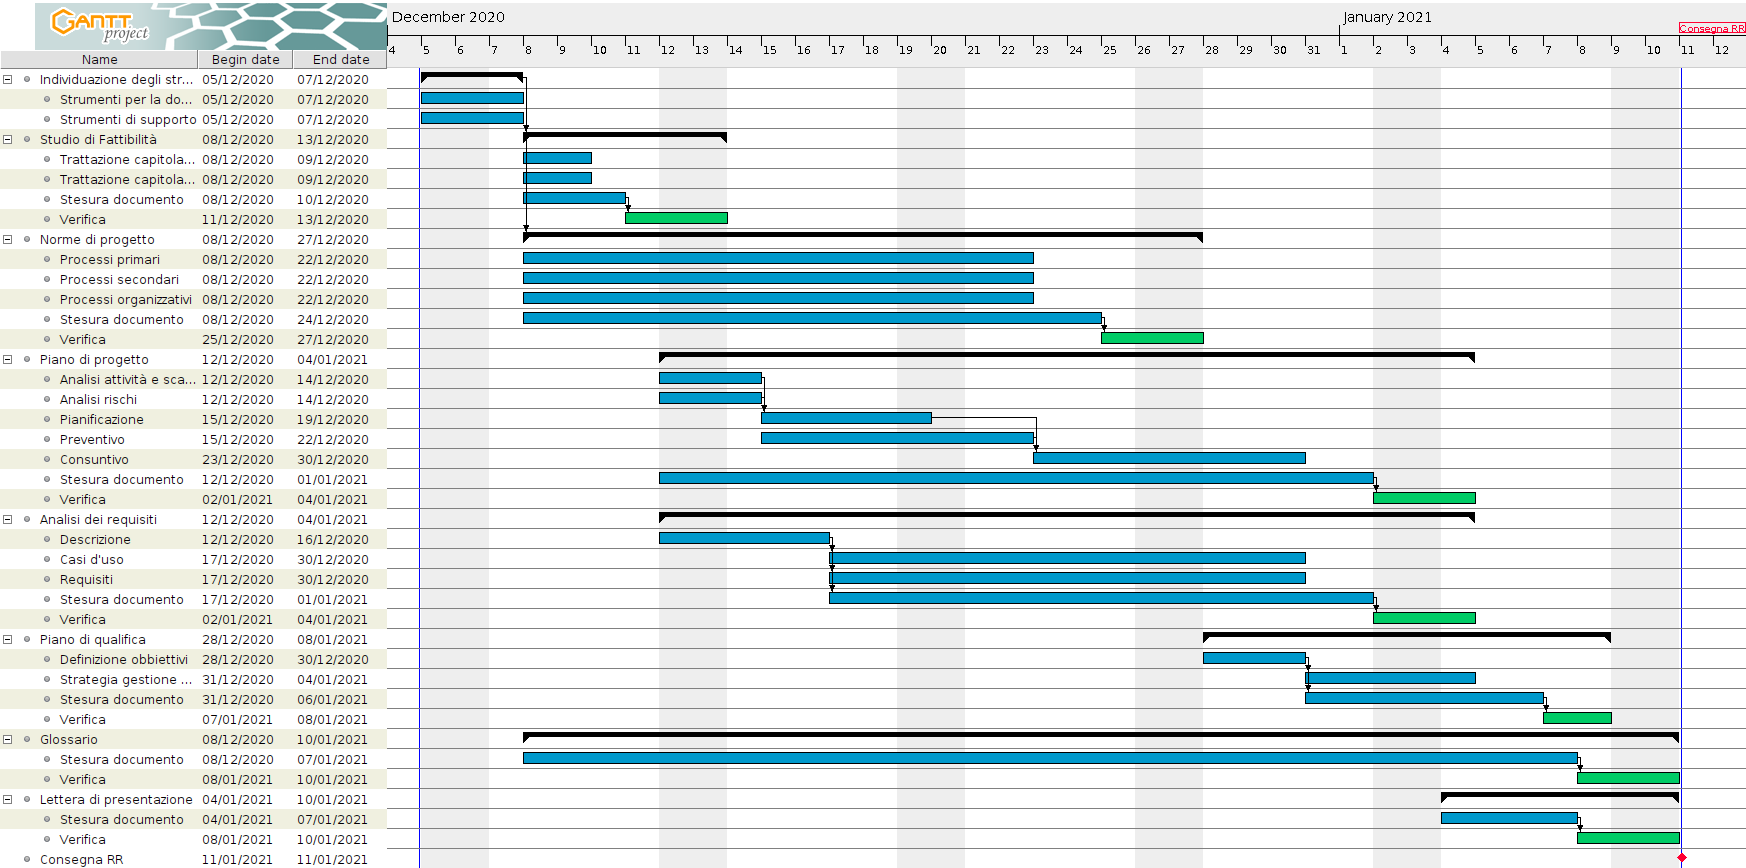
\includegraphics[width=1\linewidth]{./res/images/StrumentiRequisiti.png}
			\caption{diagramma di Gantt della fase di individuazione degli strumenti e analisi dei requisiti.}
			\label{fig:diagramma di Gantt della fase di individuazione degli strumenti e analisi dei requisiti.}
		\end{figure}
	
	
\subsection{Analisi di dettaglio}

	\textbf{periodo:} da 2021-01-12 a 2021-01-18
	\\
	\\
	Questa fase inizia con il termine della fase di Analisi dei Requisiti; il termine coincide con la data della “Revisione dei Requisiti”.
	\begin{itemize}
		\item \textbf{\glock{Analisi di Dettaglio}:} consolidamento dei requisiti richiesti, in particolare nel documento “Analisi dei Requisiti v1.00”;
		\item \textbf{Preparazione per la discussione:} realizzazione della presentazione e studio personale;
		\item \textbf{\glock{Incremento e Verifica}:} se necessario, vengono aggiornati e verificati i documenti già scritti.
	\end{itemize}  

	\subsubsection{Diagramma di Gantt: analisi di dettaglio}

		\begin{figure}[H]
			\centering
			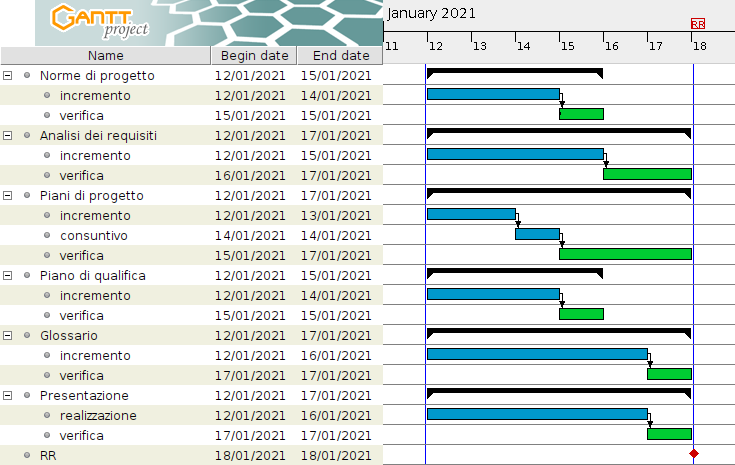
\includegraphics[width=0.7\linewidth]{./res/images/AnalisiDettaglio.png}
			\caption{diagramma di Gantt della fase di analisi di dettaglio}
			\label{fig:diagramma di Gantt della fase di analisi di dettaglio}
		\end{figure}
	
	
\subsection{Progettazione Architetturale}

	\textbf{periodo:} da 2021-01-18 a 2021-03-01 
	\\
	\\
	Questa fase comincia con la “Revisione dei Requisiti” e termina con un incontro di presentazione ufficiale con il proponente.
	\begin{itemize}
		\item \textbf{\glock{Specifica Tecnica}:} viene redatta la \glock{Specifica Tecnica} v1.0.0, che indica le scelte progettuali d’alto livello per includere al meglio le tecnologie coinvolte del prodotto finale. Il documento include i \glock{design pattern} che verranno utilizzati, l’architettura a grandi linee del prodotto e il tracciamento dei requisiti. Infine verra stilato il \glock{Proof of Concept} v1.0.0 destinato al proponente per assicurarsi il corretto sviluppo del software.
		\item \textbf{Incremento e Verifica:} se necessario, vengono aggiornati e verificati i documenti già scritti.
	\end{itemize}  

	\subsubsection{Diagramma di Gantt: progettazione architetturale}

		\begin{figure}[H]
			\centering
			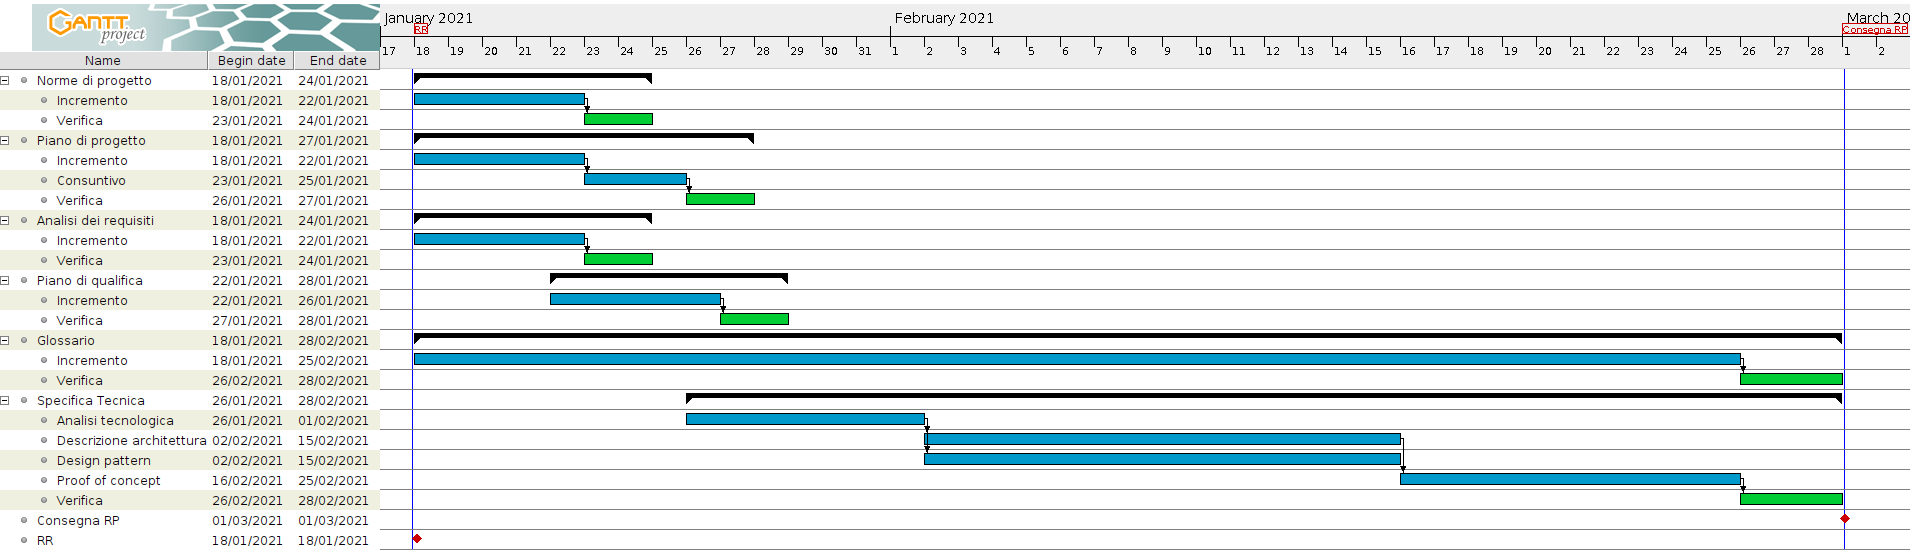
\includegraphics[width=1\linewidth]{./res/images/Architetturale.png}
			\caption{diagramma di Gantt della fase di progettazione architetturale}
			\label{fig:diagramma di Gantt della fase di progettazione architetturale}
		\end{figure}
	
	
\subsection{Progettazione di Dettaglio requisiti obbligatori e Codifica}

	\textbf{periodo:} da 2021-03-08 a 2021-03-27 
	\\
	\\
	Questa fase inizia al termine della fase di Progettazione Architetturale.
	\begin{itemize}
		\item \textbf{Definizione di prodotto:} viene stilata la “Definizione di Prodotto”, esso definirà con profondità la struttura e relazioni dei vari componenti del prodotto in relazione ai requisiti obbligatori e desiderabili;
		\item \textbf{\glock{Manuale utente}:} si inizia a stendere il manuale per fornire indicazioni su come utilizzare il prodotto;
		\item \textbf{\glock{Incremento e Verifica}:} se necessario, vengono aggiornati e verificati i documenti già scritti;
		\item \textbf{\glock{Codifica}:} viene scritto il codice con la relativa verifica.
	\end{itemize}  

	\subsubsection{Diagramma di Gantt: progettazione di dettaglio requisiti obbligatori e Codifica}

		\begin{figure}[H]
			\centering
			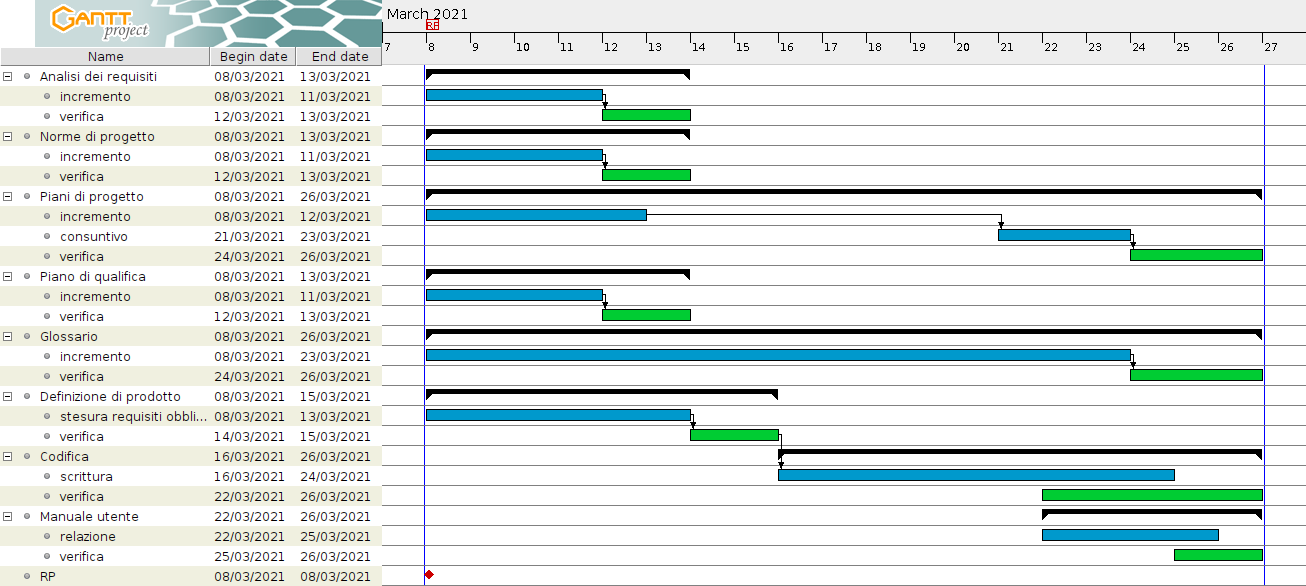
\includegraphics[width=1\linewidth]{./res/images/Obbligatori.png}
			\caption{diagramma di Gantt della fase di progettazione di dettaglio requisiti obbligatori e Codifica}
			\label{fig:diagramma di Gantt della fase di progettazione di dettaglio requisiti obbligatori e Codifica}
		\end{figure}
	
	
\subsection{Progettazione di Dettaglio requisiti opzionali e Codifica}

	\textbf{periodo:} da 2021-03-28 a 2021-04-02   

	\begin{itemize}
		\item \textbf{\glock{Definizione di prodotto}:} viene aggiornata la Definizione del Prodotto. Viene inserita la parte relativa ai requisiti opzionali;
		\item \textbf{\glock{Incremento e Verifica}:} se necessario, vengono aggiornati e verificati i documenti già scritti;
		\item \textbf{\glock{Codifica}:} viene scritto il codice con la relativa verifica.
	\end{itemize}  

	\subsubsection{Diagramma di Gantt: progettazione di dettaglio requisiti opzionali e Codifica}

		\begin{figure}[H]
			\centering
			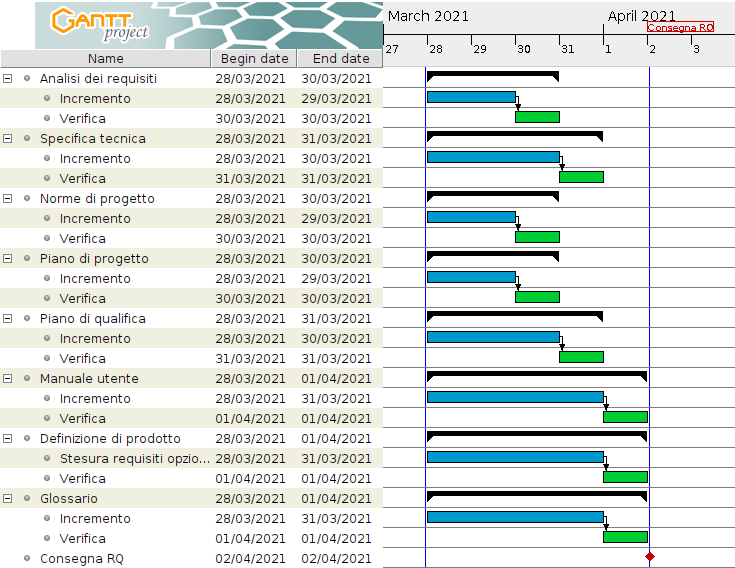
\includegraphics[width=0.7\linewidth]{./res/images/Opzionali.png}
			\caption{diagramma di Gantt della fase di progettazione di dettaglio requisiti opzionali e Codifica}
			\label{fig:diagramma di Gantt della fase di progettazione di dettaglio requisiti opzionali e Codifica}
		\end{figure}
	

\subsection{Validazione e Collaudo}

	\textbf{periodo:} da 2021-04-09 a 2021-05-03     

	\begin{itemize}
		\item \textbf{\glock{Incremento e Verifica}:} se necessario, vengono aggiornati e verificati i documenti già scritti;
		\item \textbf{\glock{Validazione}:} si verifica tramite tracciamento di aver soddisfatto i requisiti precedentemente indicati nel documento \glock{Analisi dei Requisiti} v1.00;
		\item \textbf{\glock{Collaudo}:} il prodotto viene eseguito e testato in ogni funzionalità richiesta nel capitolato;	
		\item \textbf{\glock{Consegna}:} vengono consegnati al \glock{committente} i documenti e il prodotto finito in fase di \glock{Revisione di Accettazione}.
	\end{itemize}  

	\subsubsection{Diagramma di Gantt: validazione e collaudo}

	\begin{figure}[H]
		\centering
		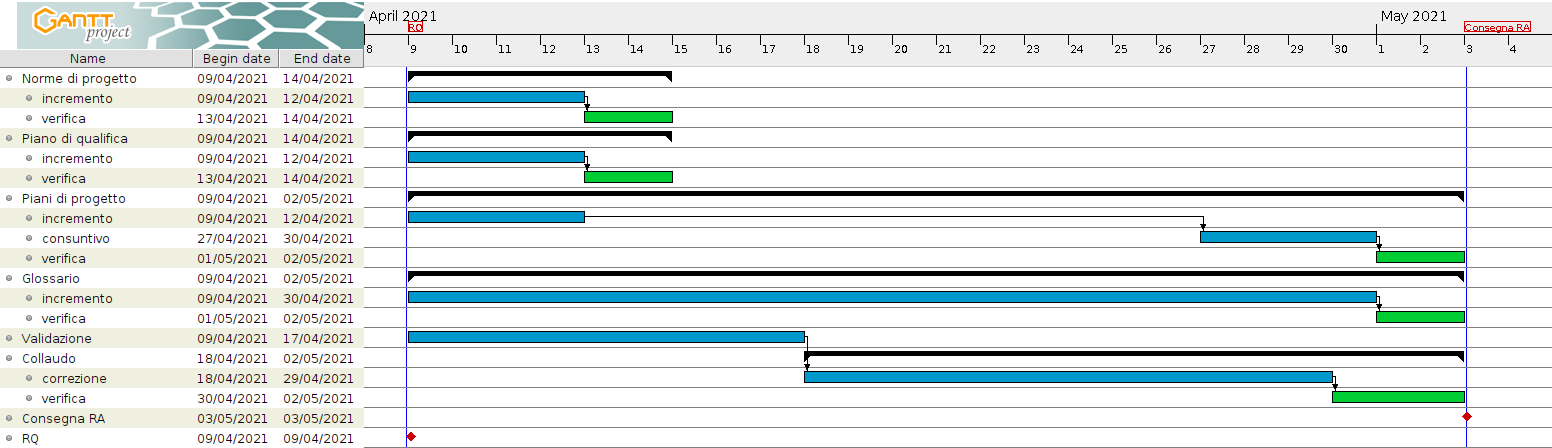
\includegraphics[width=1\linewidth]{./res/images/Validazione.png}
		\caption{diagramma di Gantt della fase di validazione e collaudo}
		\label{fig:diagramma di Gantt della fase di validazione e collaudo}
	\end{figure}
	
	